\chapter{CLaRyS prototypes}\label{chap::3}


\vfill

\minitoc

\newpage


Following the highlighted limits of ion beam therapy (see chapter~\ref{chap::1}), a collaboration of five French research institutions was established in 2008 (??) with the aim of exploring different experimental solutions for the ion range online monitoring. The research group originally involved the \enquote{\gls{ipnl}}, the \enquote{\gls{cppm}}, the \enquote{\gls{lpsc}} in Grenoble, the \enquote{\gls{lpc}} and the \enquote{\gls{creatis}} in Lyon. The collaboration focuses on the investigation of methods and detection solution for the online monitoring of ion beam range during ion beam therapy treatment, and is so called \gls{clarys}.\\
The main goal of the created collaboration is the parallel development of three gamma detection systems to be employed for ion range online monitoring purpose in the ion beam therapy field: a \gls{pet} detector, a multi-collimated gamma camera and a Compton camera.\\ The design and development of the \gls{pet} system is mainly managed by the \gls{lpc} group, which left the collaboration in 2017, and the this detection system is not treated in this thesis work.\\ 
In this chapter the two gamma cameras (multi-collimated and Compton) prototypes are described in details, and the present status of the instrumental development is presented. In the following, an entire chapter (chapter~\ref{chap::6}) is dedicated to the tests of the detectors performed on ion beams. 

\section{CLaRyS gamma cameras}\label{chap3::sec::CLaRyScameras}

The two gamma cameras under development by the CLaRyS collaboration are devoted to the detection of prompt-gamma rays emitted during ion beam treatments (see section~\ref{chap1::sec::PromptGammas}). The design of the two cameras has been optimized by different Monte Carlo simulation studies for what concerns both the detector components and the geometrical setup.\\
As already mentioned, a Compton camera is usually composed of two detector sections, a scatterer and an absorber: the CLaRyS prototype respects the standard design. In the scatterer, described in section~\ref{chap3::subsec::scatterer}, the prompt-gamma incoming ray is deflected by Compton interaction and the interaction position and energy deposited are stored. The scattered photon reaches then the absorber section, where its energy is ideally totally deposited and stored, again with the interaction position. This configuration is used to provide what is usually defined as \enquote{electronic collimation}, but a mechanical collimation is still an option for photon detection and localization. The scatterer section can be replaced by a mechanical collimator, described in section~\ref{chap3::subsec::collimator}, which selects the parallel incoming photons then absorbed by the same absorber detector (a geometrical setup adaptation is possible to optimize the detection performance and will be discussed in the following). The mechanically collimated system is called multi-collimated camera, due to the collimator multi-slit structure.\\ 
As underlined in section~\ref{chap1::sec::background}, the prompt-gamma measurements are affected by several sources of background: in particular, the signals detected by the two cameras can come from secondary particles other then prompt-gammas, like photons from positron annihilation, neutrons and protons (for beam of ions heavier then protons). One of the possible solution for background rejection is the use of \gls{tof} information (see section~\ref{chap1::sec::TOF}), requiring a further detection section dedicated to the beam tagging. A beam tagging hodoscope is being developed in parallel and can be coupled to both the gamma cameras for \gls{tof} measurements; its description is presented in section~\ref{chap3::subsec::hodoscope}.\\
A schematic view of the two prototypes is given in figure~\ref{chap3::fig::camerasScheme}.\\

\begin{figure} [!hbtp]
	\centering
	\caption{Schematic view of the two CLaRyS gamma camera prototypes: the multi-collimated camera (top) and the Compton camera (bottom).}
	\label{chap3::fig::camerasScheme}
	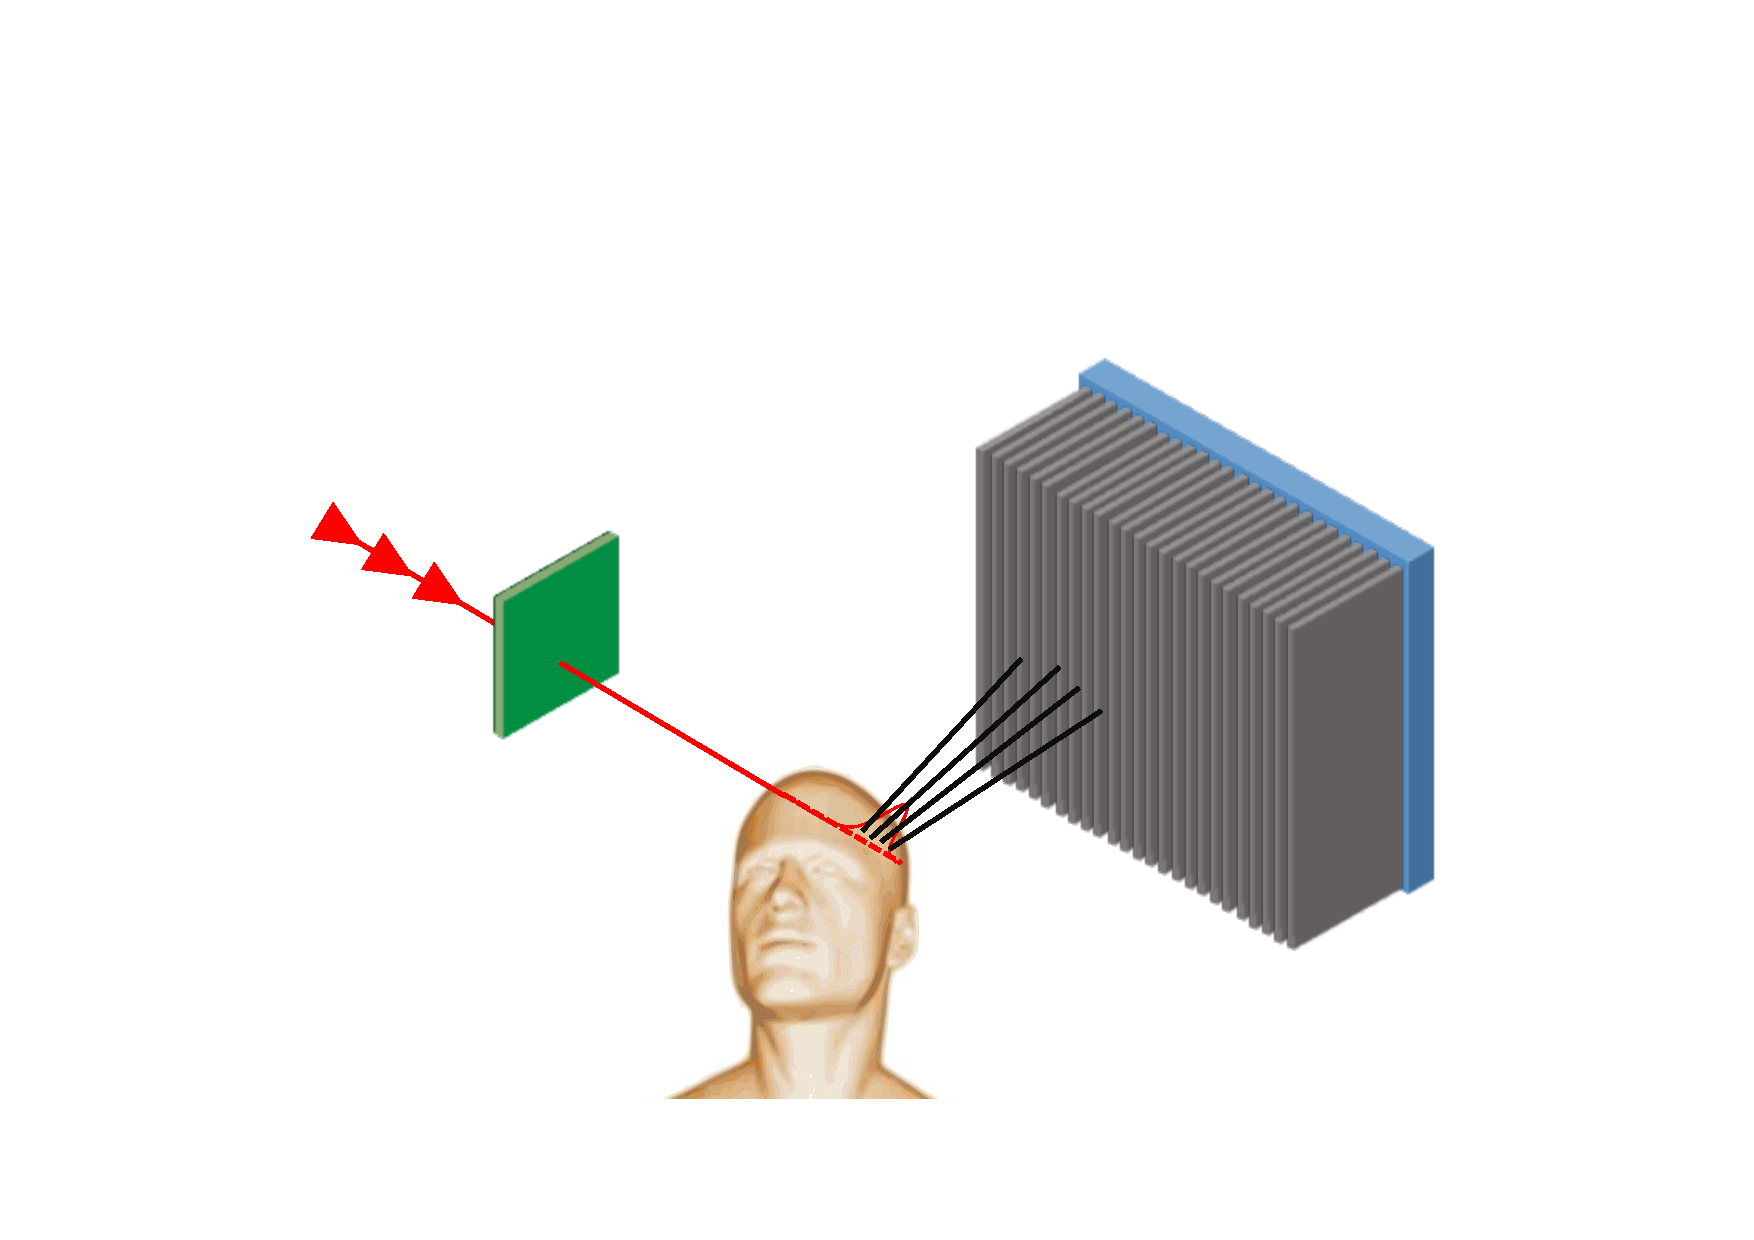
\includegraphics[width=1\textwidth]{03_GraphicFiles/chapter3_CLaRySproto/schemes/schema_Collimated_withHodo.pdf}\\
	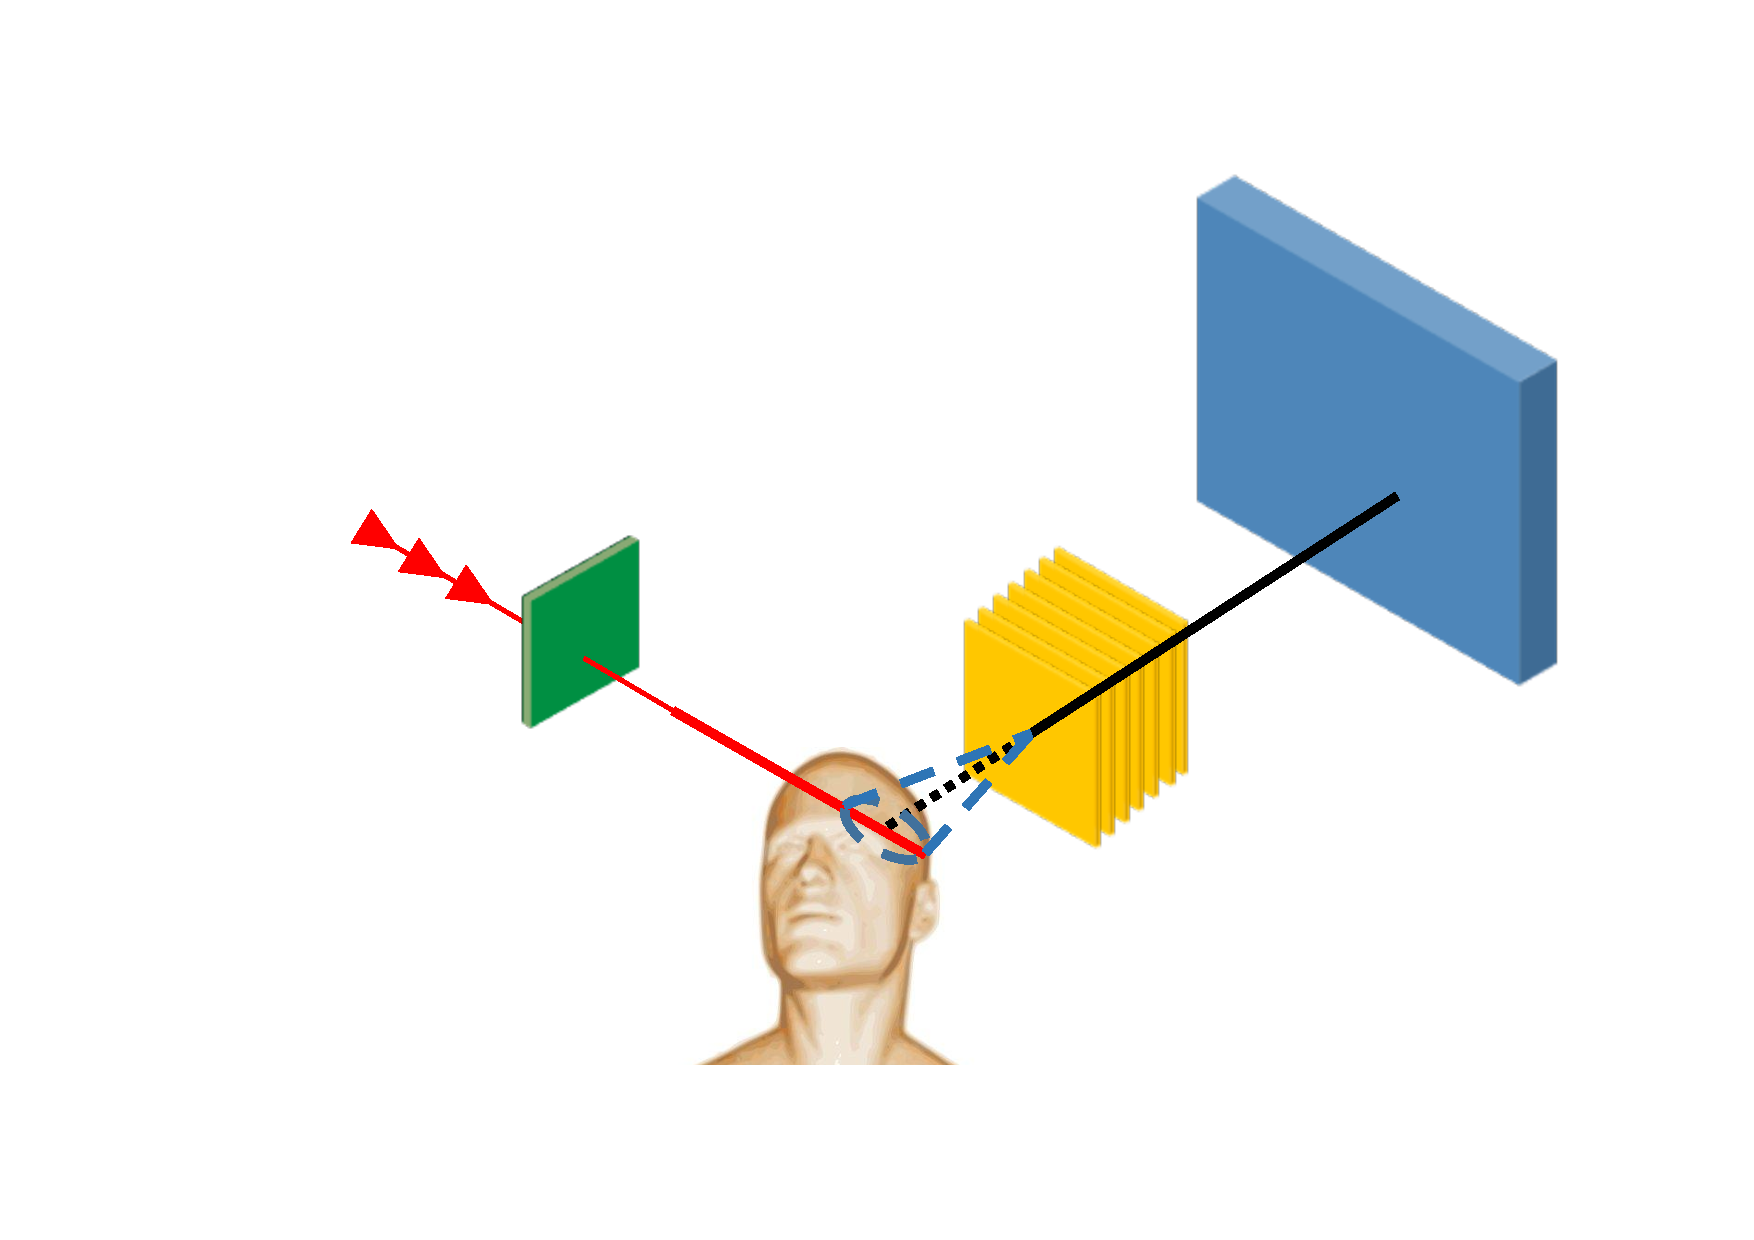
\includegraphics[width=1\textwidth]{03_GraphicFiles/chapter3_CLaRySproto/schemes/schema_Compton_withHodo.pdf}	
	\end{figure}
 

\subsection{Scatterer}\label{chap3::subsec::scatterer} 
The scatterer stack is one of the components of the Compton camera prototype. Dedicated to the photon Compton scattering, its design has been studied to optimize the Compton interaction probability in the energy range of interest and fulfill the camera requirements. The Compton events reconstruction strongly relies on the measurement of the energy deposited by the photon in its Compton interaction, mandatory to properly calculate the Compton scattering angle, which is then the aperture of the resulting Compton cone. The camera accuracy is then strictly dependent on the scattering energy resolution. At the same time, the camera efficiency is mainly due to the Compton interaction efficiency. 
 

\subsection{Collimator}\label{chap3::subsec::collimator} 

\subsection{Absorber}\label{chap3::subsec::absorber}

\subsection{Beam tagging hodoscope}\label{chap3::subsec::hodoscope}

%\subsection{Acquisition system}

%\subsection{Electronics}

%\subsection{Mechanics}

%\section{Status of instrumental development}


%\section{Next steps and perspectives}

%%%%%%%%%%%%%%%%%%%%%%%%%%%%%%%%%%%%%%%%%%%%%%%%% FROM PAPER SPECT %%%%%%%%%%%%%%%%%%%%%%%%%%%%%%%%%%%%%%%%%%%%%%%%% 
The Compton camera is composed of a scatterer part, which includes seven parallel planes of silicon detectors, 9$\times$9$\times$0.2~cm$^{3}$, with 1~cm distance between the centers of two neighboring planes, and an absorber, composed of BGO blocks of size 3.5$\times$3.5$\times$3.0~cm$^{3}$. 


The following requirements governed the choice of silicon as scattering material, and BGO as absorber~\parencite{Richard2012}:
\begin{itemize}
\item[-] optimizing the single Compton event probability, without escape of the Compton electron from the detector where it is created;
\item[-] minimizing the Doppler effect (especially important for low energy gamma rays);
\item[-] obtaining the best possible energy resolution in the scatterer;
\item[-] ensuring the best possible spatial resolution in the absorber, also thanks to the maximization of the photo-effect absorption with the highest $Z$ material.
\end{itemize}


%%%%%%%%%%%%%%%%%%%%%%%%%%%%%%%%%%%%%%%%%%%%%%%%% FROM PAPER HT %%%%%%%%%%%%%%%%%%%%%%%%%%%%%%%%%%%%%%%%%%%%%%%%% 

\clearpage
%\printbibliography[heading=subbibintoc]
